\section{Durchführung}
\label{sec:Durchführung}


Für den Versuch wird ein Aufbau gemäß Abbildung \ref{fig:aufbau} verwendet.

\begin{figure}
    \centering
    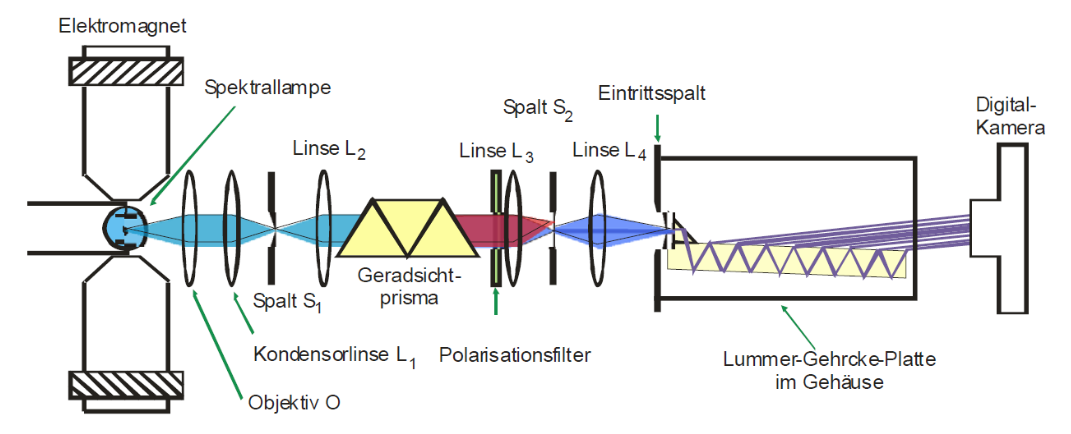
\includegraphics[width=\textwidth]{Bilder/Aufbau.PNG}
    \caption{Schematischer Versuchsaufbau.}
    \label{fig:aufbau}
\end{figure}

Für eine möglichst genaue Messung muss der Aufbau zunächst justiert werden. Die Justage wird an der Cd-Lampe begonnen und der Reihenfolge der Bauteile nach durchgeführt. 
Als erstes wird das Licht der Cd-Lampe über ein Objektiv und einer Linse scharf auf den ersten Spalt $S_1$ abgebildet.
Daraufhin wird das Licht in der Linse $L_2$ so gebrochen, dass ein möglichst paralleles Lichtbündel entsteht, welches dann mit wenig Verlust in das Geradsichtprisma fällt. Dazu sollte der Durchmesser des Lichtsbündels die größe des Prismas nicht übersteigen. 
Über die Linse $L_3$ werden die Lichtstrahlen, die das Prisma verlassen, scharf auf den Spalt $S_2$ abgebildet. Über den Spalt kann dann eine Selektion der einzelnen Spektrallinien vorgenommen werden. Im Versuch wird mit der roten Linie begonnen. Über die Justage der Linse $L_4$ wird ein scharfes Bild auf die Lummer-Gehrcke-Platte geworfen. Auch hier wird darauf geachtet, dass das Bild der Größe des Eintritts-Prismas entspricht. 
Nun wird ein Polarisator in dem Strahlengang platziert, welcher, je nach Stellung, den jeweiligen Übergang ($\Delta m = \pm1,0$) ausblendet.
Am Ende des Aufbaus ist eine Kamera angebracht, mit der die aufgespalteten Linien fotografiert werden können. Nach erneuter Einstellung des Spaltes $S_2$ und jeweiliger Nachjustage der darauf folgenden Bauteile werden die jeweiligen Bilder der blauen Linie aufgenommen.


 %Was wurde gemessen bzw. welche Größen wurden variiert?